\subsection{Descrição de \textit{hardware}}\label{subsec:hardware}

O sistema é composto por uma arquitetura híbrida que divide as responsabilidades entre um microprocessador Broadcom BCM2837 hospedado numa placa Raspberry pi 3B e realizará as tarefas de alto nível, e um microcontrolador STM32G070 dedicado ao controle em tempo real dos dispositivos físicos da esteira. O diagrama de blocos apresentado abaixo mostra de forma simplificada a arquitetura do sistema:


   \begin{figure}[h!]
    \centering
    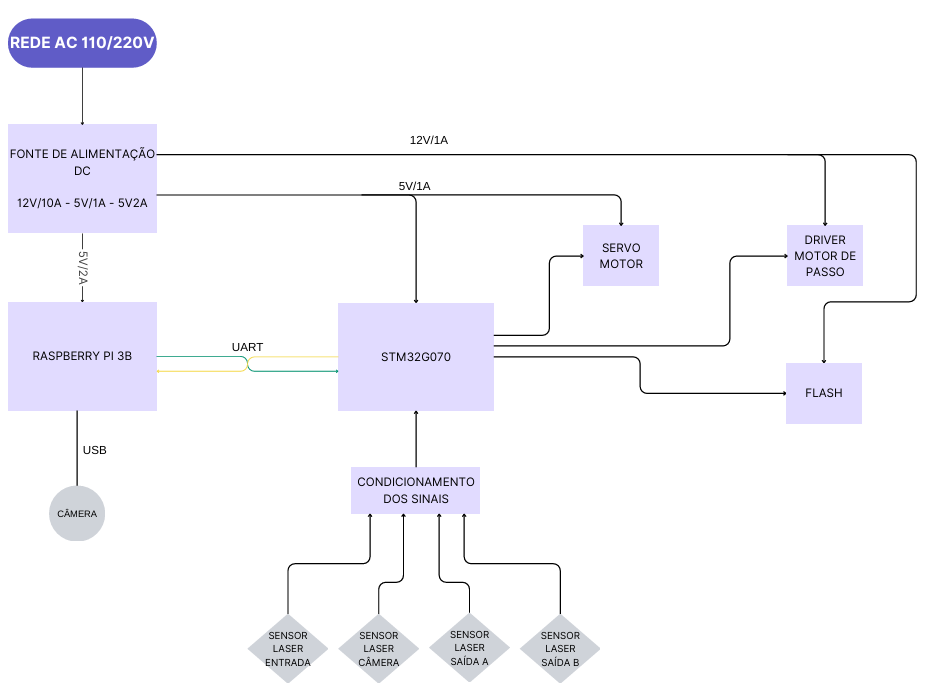
\includegraphics[width=0.75\linewidth]{figuras/Diagrama_blocos_HW.png}
    \caption{Diagrama de blocos do hardware}
    \label{fig:Diag_blocks}
\end{figure}




A placa Raspberry pi 3B foi escolhida devido a ampla documentação disponível na internet e pela acessibilidade ao hardware, pois além de ser um modelo disponível no laboratório da universidade, um dos integrantes da dupla já possuia uma em prontidão para iniciar os desenvolvimentos do software.

A câmera utilixada para a leitura e processamento da imagem é uma webcam genérica da marca Multilaser, que funciona com USB. A escolha dela foi motivada pela ausência da necessidade de drivers proprietários para o correto funcionamento com o linux embarcado e pela disponibilidade para o projeto.

O microcontrolador STM32G070 foi escolhido devido a sua variedade de periféricos disponíveis para a aplicação, tais como comunicação UART, Timers de uso geral e o recurso de DMA - Direct Memory Access, que permite processar informações obtidas pelos periféricos sem ocupar a CPU do microcontrolador. Além dessas caracteristicas vantajosas para o controle do hardware da esteira em tempo real, o STM32G070 possui uma interface integrada de desenvolvimento suportada pela STmicroelectronics, que é referência mundial na fabricação e suporte de microcontroladores para a indústria.

\begin{figure}[h!]
    \centering
    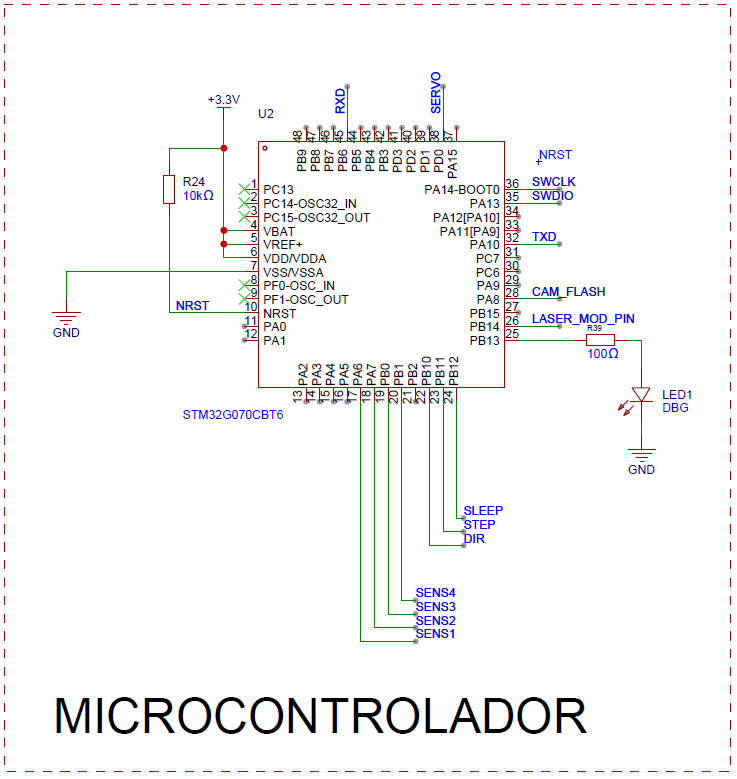
\includegraphics[width=0.75\linewidth]{figuras/Esquematico_microcontrolador.png}
    \caption{Esquemático STM32}
    \label{fig:sch_stm32}
\end{figure}

Como sistema motor do tapete da esteira, foi utilizado um motor de passo NEMA 22 controlado por um driver de motor de passo A4988. Esses componentes foram escolhidos devido a disponibilidade e a baixa complexidade operacional para o controle do driver.

\begin{figure}[h!]
    \centering
    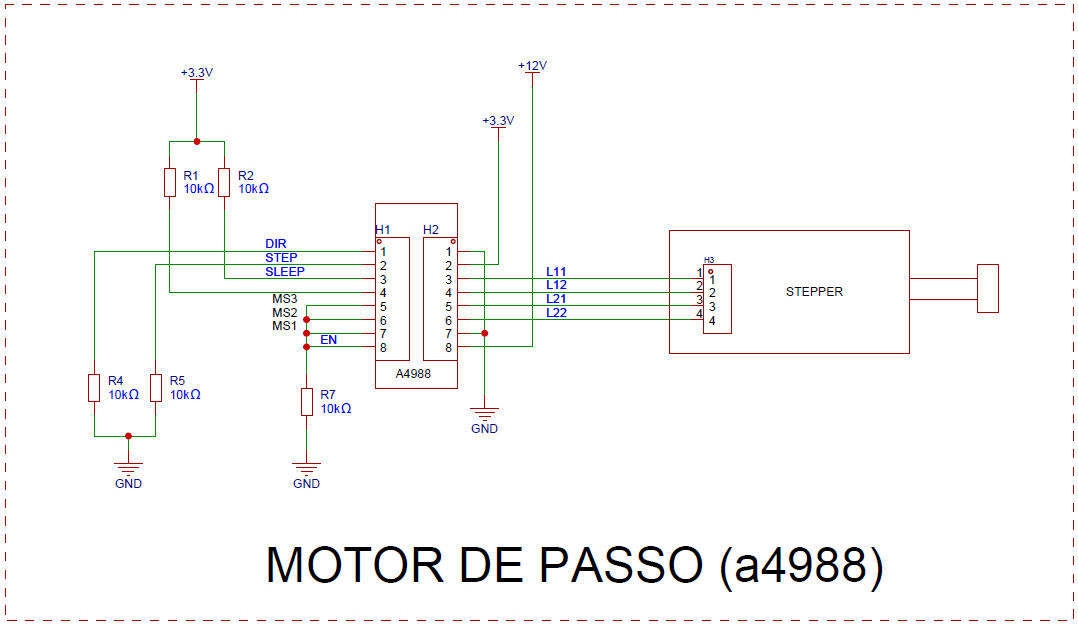
\includegraphics[width=0.85\linewidth]{figuras/Motor_de_passo_driver.png}
    \caption{Esquemático motor de passo}
    \label{fig:sch_motor_passo}
\end{figure}

Como motor da cancela foi utilizado um servomotor ES08MA, que foi selecionado devido a disponibilidade para o projeto e elevado torque comparado ao servo motor SG90.

\begin{figure}[h!]
    \centering
    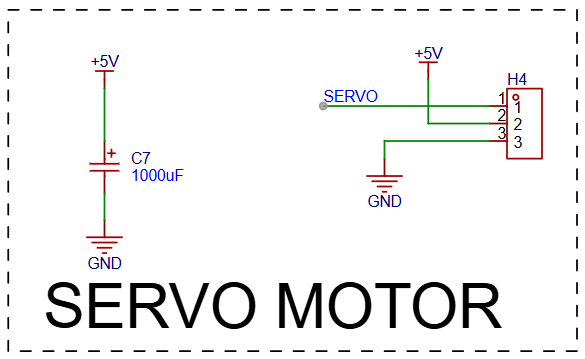
\includegraphics[width=0.75\linewidth]{figuras/servo_motor.png}
    \caption{Esquemático servo motor}
    \label{fig:sch_servo_motor}
\end{figure}

Os sensores laser foram projetados para serem o mais simples possível e de forma que o circuito eletrônico fosse viável de se fabricar artesanalmente (não foi desenhada uma placa de circuito impresso para este projeto, o circuiot foi montado em breakout boards com solda a mão para agilidade e baixo custo instantâneo). O funcionamento dos sensores ocorre a partir de um princípio de detecção síncrona por ausência de portadora. Um laser modula seu feixe na mesma frequência gerada pelo STM32. O feixe incide sobre um LDR que, após condicionamento de sinal com amplificadores operacionais, entrega ao STM32 um sinal digital pulsado na faixa de 0 a 3,3 V com frequência idêntica à portadora [CITAR CIRCUITO AQUI]. Quando um objeto interrompe o feixe, a ausência do sinal pulsado [CITAR SAIDA EM NIVEL HIGH AQUI] é interpretada pelo firmware como presença de objeto em frente ao sensor.

  COLOCAR CAPTURA DE TELA DO SCH COM APENAS UMA SEÇÃO DO CIRCUITO DO LASER (A DE BAIXO QUE MOSTRA O MOSFET ACIONANDO O LASER)

  

Para auxiliar a visualização do código QR pela câmera, o sistema conta também com um flash, que aciona seis leds de uma fita de leds da cor 4000k. A escolha da cor foi considerada levando em conta a similaridade com a luz ambiente, que ofereceu um resultado melhor para a visualização na câmera do que a cor 6500K. O circuito de acionamento da luminária é feito 


 COLCOAR CAPTURA DE TELA DO CIRCUITO DE ACIOANEMTNO DA LUMINÁRIA
    
O esquemático completo da placa de circuito montada para o projeto pode ser observado nos anexos.

Para realizar a montagem completa do sistema foi elaborada uma lista de materiais A Tabela \ref{tab:BOM} (Bill of Materials):


% === ELETRÔNICA ================================================
\begin{table}[!htpb]
\caption{Lista de materiais -- Eletrônica.}
\label{tab:BOM_eletro}
\centering
\renewcommand{\arraystretch}{0.85}
\small
\begin{tabular}{lcc}
\hline
\textbf{Componente} & \textbf{Preço unit. (R\$)} & \textbf{Qtd.} \\
\hline
Raspberry Pi 3B                        & --   & 1  \\
Webcam genérica                        & --   & 1  \\
ST-Link V2                             & --   & 1  \\
STM32G070                              & 5,50 & 1  \\
Driver A4988                           & 18,00 & 1  \\
AMS1117-3.3                            & 1,00 & 1  \\
Módulo Buck LM2596S                    & 15,00 & 1  \\
AmpOp LM324                            & 3,50 & 1  \\
Diodo 1N4007                           & 0,50 & 1  \\
Capacitor eletrolítico 1000\,$\mu$F    & 0,50 & 1  \\
Motor de passo NEMA 22                 & 60,00 & 1  \\
Servomotor ES08MA                      & 25,00 & 1  \\
MOSFET BUK9Y14                         & 1,00 & 2  \\
Transistor BJT BC547B                  & 0,20 & 4  \\
Resistor 100\,$\Omega$                 & 0,10 & 3  \\
Resistor 1\,k$\Omega$                  & 0,10 & 12 \\
Resistor 1k5\,$\Omega$                 & 0,10 & 4  \\
Resistor 2k2\,$\Omega$                 & 0,10 & 4  \\
Resistor 10\,k$\Omega$                 & 0,10 & 8  \\
Resistor 100\,k$\Omega$                & 0,10 & 4  \\
LDR 10\,k$\Omega$                      & 0,50 & 4  \\
Laser com ajuste focal                 & 1,00 & 4  \\
Capacitor 100\,nF                      & 0,10 & 6  \\
Fio coaxial (sensores LDR)             & 10,00 & 2\,m \\
Fio 22\,AWG vermelho (lasers)          & 1,50 & 2\,m \\
Fio 22\,AWG azul (lasers)              & 1,50 & 2\,m \\
Fio 22\,AWG preto (servo)              & 1,50 & 1\,m \\
Fio 22\,AWG branco (servo)             & 1,50 & 1\,m \\
Fio 22\,AWG amarelo (servo)            & 1,50 & 1\,m \\
Conector Molex KK macho 2 terminais    & 0,10 & 8  \\
Conector Molex KK macho 3 terminais    & 0,15 & 2  \\
Conector Molex KK fêmea 2 terminais    & 0,10 & 8  \\
Conector Molex KK fêmea 3 terminais    & 0,15 & 2  \\
\hline
\textbf{Total (itens com preço definido)} & \textbf{163,80} & \\
\hline
\end{tabular}
\end{table}

% === MECÂNICA ==================================================
\begin{table}[!htpb]
\caption{Lista de materiais -- Mecânica.}
\label{tab:BOM_mec}
\centering
\renewcommand{\arraystretch}{0.85}
\small
\begin{tabular}{lcc}
\hline
\textbf{Componente} & \textbf{Preço unit. (R\$)} & \textbf{Qtd.} \\
\hline
\multicolumn{3}{l}{\textit{Fixação e estrutura}} \\
\hline
Parafuso para madeira                              & 0,01  & 64 \\
Arruela galvanizada (ajuste dos rolos)             & 0,10  & 2  \\
Pino de eixo                                       & 1,50  & 3  \\
Rolamento 608                                      & 5,00  & 3  \\
Super cola Tek Bond 793 (20\,g)                    & 20,00 & 1  \\
Abraçadeiras de nylon (pacote)                     & 10,00 & 1  \\
Chapa de PVC 15\,$\times$\,55\,cm                 & --    & 1  \\
Cano de PVC $\frac{1}{2}$\,pol $\times$ 12,5\,cm  & --    & 2  \\
\hline
\multicolumn{3}{l}{\textit{Peças 3D -- Estrutural (P. Caleb)}} \\
\hline
\texttt{Wood\_stitches}         & $\ast$ & 3 \\
\texttt{Apoio\_Base}            & $\ast$ & 8 \\
\texttt{Suporte\_Motor}         & $\ast$ & 1 \\
\texttt{Trava\_Suporte\_Motor}  & $\ast$ & 1 \\
\texttt{Suporte\_Parafuso}      & $\ast$ & 3 \\
\texttt{Tampa\_Rolo\_Motor}     & $\ast$ & 1 \\
\texttt{Tampa\_Rolo\_Rolamento} & $\ast$ & 3 \\
\texttt{Suporte\_Mesa}          & $\ast$ & 6 \\
\texttt{Lateral\_esq\_rampa}    & $\ast$ & 1 \\
\texttt{Lateral\_dir\_rampa}    & $\ast$ & 1 \\
\hline
\multicolumn{3}{l}{\textit{Peças 3D -- Sensoriamento/Eletrônica (F. Castro)}} \\
\hline
\texttt{Cancela\_servo}               & $\ast$ & 1 \\
\texttt{Suporte\_Servo}               & $\ast$ & 1 \\
\texttt{Suporte\_STlink}              & $\ast$ & 1 \\
\texttt{Suporte\_laser\_focal} (mesa) & $\ast$ & 3 \\
\texttt{Suporte\_LDR} (mesa)          & $\ast$ & 3 \\
\texttt{Suporte\_laser\_Rampa}        & $\ast$ & 1 \\
\texttt{Suporte\_LDR\_Rampa}          & $\ast$ & 1 \\
\texttt{Suporte\_flash}               & $\ast$ & 2 \\
\texttt{Suporte\_poste\_camera}       & $\ast$ & 2 \\
\texttt{Suporte\_camera}              & $\ast$ & 1 \\
\texttt{Case RBPi 3B} (MakerWorld)    & $\ast$ & 1 \\
\hline
Filamento PLA (1\,kg -- rateio total) & 120,00 & 1 \\
\hline
\textbf{Total (itens com preço definido)} & \textbf{170,34} & \\
\hline
\multicolumn{3}{l}{%
  \footnotesize $\ast$ Impressas em impressora própria; custo rateado} \\
\multicolumn{3}{l}{%
  \footnotesize no filamento (1\,kg a R\$\,120,00 cobriu todas as peças com sobra).} \\
\hline
\end{tabular}
\end{table}










